\documentclass[11pt,twoside,a4paper]{scrartcl}
	\usepackage[english]{babel}
	\usepackage{amsmath}
	\usepackage{amsthm}
	\usepackage{amssymb}
	\usepackage{hyperref}
	\usepackage{graphicx}
	\usepackage{listings}
	\usepackage{color}

	\usepackage[nameinlink,capitalise]{cleveref}

	%Link colors
	\usepackage{xcolor}
	\definecolor{dark-red}{rgb}{0.4,0.15,0.15}
	\definecolor{dark-blue}{rgb}{0.15,0.15,0.4}
	\definecolor{medium-blue}{rgb}{0,0,0.5}
	\hypersetup{
		colorlinks, linkcolor={dark-blue},
		citecolor={dark-blue}, urlcolor={medium-blue}
	}

	\definecolor{mycomment}{rgb}{0.3,0.7,0.8}
	\definecolor{mygray}{rgb}{0.5,0.5,0.5}
	\definecolor{lightgray}{rgb}{0.95,0.95,0.95}
	\definecolor{mymauve}{rgb}{0.58,0,0.82}

	\lstset{
	  backgroundcolor=\color{lightgray},
	  basicstyle=\footnotesize,
	  breakatwhitespace=false,
	  breaklines=true,
	  captionpos=b,
	  commentstyle=\color{mycomment},
	  escapeinside={\%*}{*)},
	  extendedchars=true,
	  keepspaces=true,
	  keywordstyle=\color{black}\bfseries,
	  language=matlab,
	  numbers=left,
	  numbersep=5pt,
	  numberstyle=\tiny\color{mygray},
	  rulecolor=\color{black},
	  showspaces=false,
	  showstringspaces=false,
	  showtabs=false,
	  stringstyle=\color{mymauve},
	  tabsize=2,
	  title=\lstname
	}

	%Pseudocode
	\usepackage{algorithm}
	\usepackage[noend]{algpseudocode}

	% Euro symbol
	\usepackage[official]{eurosym}

	% SI-units
	\usepackage{siunitx}

	% Circuit drawing
	\usepackage[siunitx]{circuitikz}

	\title{A Fiber Tap Proof of Concept}
	\subtitle{Tapping Communications on the Cheap}
	\author{
		Eddie Schoute, 4101790\\
		Alex van Rijs, ???
	}

\begin{document}
\maketitle

\begin{abstract}
	\noindent Network security is a very important concept in today's information society.
	With the heavy reliance on data communications, comes also a responsibility for its security.
	While fiber cables are an improvement over traditional copper with respect to tapping,
	it is still very possible to tap these cables as we will show in this paper.
	We will give a proof of concept of tapping fiber communications ``on the cheap'',
	using less than \euro{}$20$ in hardware materials.
	As such we recommend that confidential data communication needs to be encrypted,
	even when using fiber optic cables.
\end{abstract}

\section{Introduction}
	%Subject introduction
	Terabytes of data are being exchanged over fiber optic cables every day and user rely on their security.
	As can be shown with the recent controversy surrounding the tapping of Google and Yahoo network infrastructure~\cite{googleyahootap},
	the pure physical layer of communications is still assumed to be secure.

	%Research question and contributions
	While it is better known that copper taps are easy to install, fiber optic communications are harder to tap.
	In this paper we will investigate the possible ways an intruder may use to tap fiber optic links.
	We we also look into bringing these methods into practice, by supplying a proof of concept implementation.

\section{Design}
	% Some background research and interesting stuff that we used

\section{Proof of Concept}
	For the proof of concept we discern three parties, the sender, receiver and tapper.
	The sender and receiver are legitimate communication parties,
	while the tapper tries to gain access to the communications between them.
	For the proof of concept we used Arduino boards for simple prototyping and some other hardware
	that we will discuss in later sections.
	First we set up a fiber optic communication link between sender and receiver,
	after which we installed the tapper.

	\subsection{Fiber Communication}
		At first we tried to set up a communication using two Arduinos, an LED with a wavelength of about \SI{650}{\micro\meter},
		a fiber cable, a lens and a photoresistor.
		We immediately noticed that simply shining the LED into the cable would not work,
		because not enough light enters the cable using this method.
		When using a lens to focus the light on the cable entrance,
		the results were better but still not satisfactory.
		Only after consulting with the Optics department did we give up on using this method
		and ordered a fiber communication kit.

		The kit included a transmitter, receiver, a fiber cable with connectors and some other materials we did not use.
		The adjoining data sheet includes a circuit for simple \SI{40}{\kilo Bd} communication link,
		which we used for building a basic communication link~\cite[p.15]{avagokit},
		see \cref{fig:transmitter}.

		\begin{figure}
			\centering
			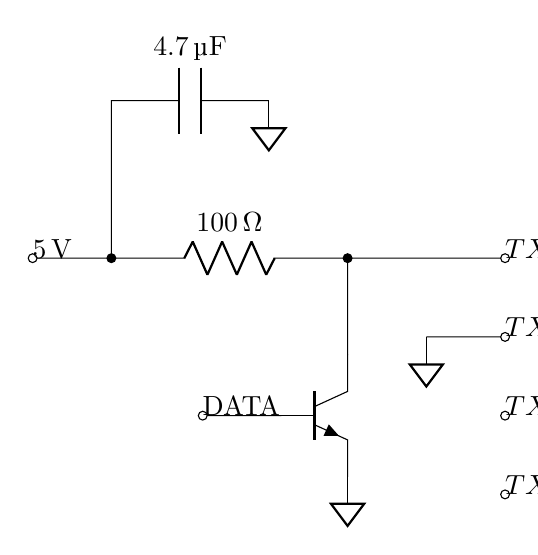
\begin{tikzpicture}
			  \draw
			  (0,5) node[ocirc] {\SI{5}{\volt}}
			  to (1,5) node[circ] (input) {}
			  to ++(0,2)
			  to[C, l={\SI{4.7}{\micro\farad}}] ++(2,0)
			  node[sground] {}

			  (input) to[R, l={\SI{100}{\ohm}}] ++(3,0) node[circ] (transmitter) {}
			  ++(0,-2) node[npn] (npn) {}
			  (transmitter) to (npn.collector) {}

			  (npn.base) to ++(-1,0) node[ocirc] {DATA}
			  (npn.emitter) node[sground] {}

			  (transmitter) to ++(2,0) node[ocirc] (tx1) {$TX_1$}
			  ++(0,-1) node[ocirc] (tx2) {$TX_2$}
			  to ++(-1,0) node[sground] {}
			  (tx2) ++(0,-1) node[ocirc] {$TX_3$}
			  ++(0,-1) node[ocirc] {$TX_4$}
			  ;
			\end{tikzpicture}
			\caption{Circuit of the transmitter}
			\label{fig:transmitter}
		\end{figure}

\section{Conclusion}

\bibliographystyle{abbrv}
\bibliography{bibl}

\end{document}
